\documentclass{book}
\usepackage[a4paper,top=2.5cm,bottom=2.5cm,left=2.5cm,right=2.5cm]{geometry}
\usepackage{makeidx}
\usepackage{natbib}
\usepackage{graphicx}
\usepackage{multicol}
\usepackage{float}
\usepackage{listings}
\usepackage{color}
\usepackage{ifthen}
\usepackage[table]{xcolor}
\usepackage{textcomp}
\usepackage{alltt}
\usepackage{ifpdf}
\ifpdf
\usepackage[pdftex,
            pagebackref=true,
            colorlinks=true,
            linkcolor=blue,
            unicode
           ]{hyperref}
\else
\usepackage[ps2pdf,
            pagebackref=true,
            colorlinks=true,
            linkcolor=blue,
            unicode
           ]{hyperref}
\usepackage{pspicture}
\fi
\usepackage[utf8]{inputenc}
\usepackage{polski}
\usepackage[T1]{fontenc}

\usepackage{mathptmx}
\usepackage[scaled=.90]{helvet}
\usepackage{courier}
\usepackage{sectsty}
\usepackage{amssymb}
\usepackage[titles]{tocloft}
\usepackage{doxygen}
\lstset{language=C++,inputencoding=utf8,basicstyle=\footnotesize,breaklines=true,breakatwhitespace=true,tabsize=4,numbers=left }
\makeindex
\setcounter{tocdepth}{3}
\renewcommand{\footrulewidth}{0.4pt}
\renewcommand{\familydefault}{\sfdefault}
\hfuzz=15pt
\setlength{\emergencystretch}{15pt}
\hbadness=750
\tolerance=750
\begin{document}
\hypersetup{pageanchor=false,citecolor=blue}
\begin{titlepage}
\vspace*{7cm}
\begin{center}
{\Large Benchmark }\\
\vspace*{1cm}
{\large Wygenerowano przez Doxygen 1.8.3.1}\\
\vspace*{0.5cm}
{\small N, 2 mar 2014 13:40:01}\\
\end{center}
\end{titlepage}
\clearemptydoublepage
\pagenumbering{roman}
\tableofcontents
\clearemptydoublepage
\pagenumbering{arabic}
\hypersetup{pageanchor=true,citecolor=blue}
\chapter{Strona główna}
\label{index}\hypertarget{index}{}\hypertarget{index_opis}{}\section{Opis programu}\label{index_opis}
Program mierzy czas wykonania algorytmu, który mnoży każdy element wektora przez 2. 
\chapter{Indeks przestrzeni nazw}
\section{Lista przestrzeni nazw}
Tutaj znajdują się wszystkie przestrzenie nazw wraz z ich krótkimi opisami\-:\begin{DoxyCompactList}
\item\contentsline{section}{\hyperlink{namespace_generate_input}{Generate\-Input} }{\pageref{namespace_generate_input}}{}
\end{DoxyCompactList}

\chapter{Indeks hierarchiczny}
\section{Hierarchia klas}
Ta lista dziedziczenia posortowana jest z grubsza, choć nie całkowicie, alfabetycznie\-:\begin{DoxyCompactList}
\item \contentsline{section}{Benchmark$<$ Problem\-Type $>$}{\pageref{class_benchmark}}{}
\item \contentsline{section}{Benchmark\-Data}{\pageref{struct_benchmark_data}}{}
\item \contentsline{section}{Problem}{\pageref{class_problem}}{}
\begin{DoxyCompactList}
\item \contentsline{section}{Standard\-Problem$<$ Input\-Data\-Type, Output\-Data\-Type $>$}{\pageref{class_standard_problem}}{}
\item \contentsline{section}{Standard\-Problem$<$$>$}{\pageref{class_standard_problem}}{}
\begin{DoxyCompactList}
\item \contentsline{section}{Multiply\-By2}{\pageref{class_multiply_by2}}{}
\end{DoxyCompactList}
\end{DoxyCompactList}
\item \contentsline{section}{Timer}{\pageref{class_timer}}{}
\end{DoxyCompactList}

\chapter{Indeks klas}
\section{Lista klas}
Tutaj znajdują się klasy, struktury, unie i interfejsy wraz z ich krótkimi opisami\-:\begin{DoxyCompactList}
\item\contentsline{section}{\hyperlink{class_benchmark}{Benchmark$<$ Problem\-Type $>$} \\*Klasa pozwalająca na testowanie algorytmów }{\pageref{class_benchmark}}{}
\item\contentsline{section}{\hyperlink{struct_benchmark_data}{Benchmark\-Data} \\*Struktura przechowująca informacje o pojedynczym teście wydajności }{\pageref{struct_benchmark_data}}{}
\item\contentsline{section}{\hyperlink{class_multiply_by2}{Multiply\-By2} \\*Klasa reprezentuje algorytm mnożenia tablicy przez 2 }{\pageref{class_multiply_by2}}{}
\item\contentsline{section}{\hyperlink{class_problem}{Problem} \\*Abstrakcyjna klasa reprezentująca problem algorytmiczny }{\pageref{class_problem}}{}
\item\contentsline{section}{\hyperlink{class_standard_problem}{Standard\-Problem$<$ Input\-Data\-Type, Output\-Data\-Type $>$} \\*Klasa definiuje standardowy problem algorytmiczny }{\pageref{class_standard_problem}}{}
\item\contentsline{section}{\hyperlink{class_timer}{Timer} \\*Klasa mierząca długość interwału czasu }{\pageref{class_timer}}{}
\end{DoxyCompactList}

\chapter{Indeks plików}
\section{Lista plików}
Tutaj znajduje się lista wszystkich plików z ich krótkimi opisami\-:\begin{DoxyCompactList}
\item\contentsline{section}{/home/mochman/\-Politechnika/\-P\-A\-M\-S\-I/benchmark-\/multiply-\/by-\/2/prj/inc/\hyperlink{_benchmark_8hpp}{Benchmark.\-hpp} }{\pageref{_benchmark_8hpp}}{}
\item\contentsline{section}{/home/mochman/\-Politechnika/\-P\-A\-M\-S\-I/benchmark-\/multiply-\/by-\/2/prj/inc/\hyperlink{_multiply_by2_8hpp}{Multiply\-By2.\-hpp} }{\pageref{_multiply_by2_8hpp}}{}
\item\contentsline{section}{/home/mochman/\-Politechnika/\-P\-A\-M\-S\-I/benchmark-\/multiply-\/by-\/2/prj/inc/\hyperlink{_problem_8hpp}{Problem.\-hpp} }{\pageref{_problem_8hpp}}{}
\item\contentsline{section}{/home/mochman/\-Politechnika/\-P\-A\-M\-S\-I/benchmark-\/multiply-\/by-\/2/prj/inc/\hyperlink{_standard_problem_8hpp}{Standard\-Problem.\-hpp} }{\pageref{_standard_problem_8hpp}}{}
\item\contentsline{section}{/home/mochman/\-Politechnika/\-P\-A\-M\-S\-I/benchmark-\/multiply-\/by-\/2/prj/inc/\hyperlink{_timer_8hpp}{Timer.\-hpp} }{\pageref{_timer_8hpp}}{}
\item\contentsline{section}{/home/mochman/\-Politechnika/\-P\-A\-M\-S\-I/benchmark-\/multiply-\/by-\/2/prj/src/\hyperlink{main_8cpp}{main.\-cpp} }{\pageref{main_8cpp}}{}
\item\contentsline{section}{/home/mochman/\-Politechnika/\-P\-A\-M\-S\-I/benchmark-\/multiply-\/by-\/2/prj/src/\hyperlink{_multiply_by2_8cpp}{Multiply\-By2.\-cpp} }{\pageref{_multiply_by2_8cpp}}{}
\item\contentsline{section}{/home/mochman/\-Politechnika/\-P\-A\-M\-S\-I/benchmark-\/multiply-\/by-\/2/prj/src/\hyperlink{_timer_8cpp}{Timer.\-cpp} }{\pageref{_timer_8cpp}}{}
\item\contentsline{section}{/home/mochman/\-Politechnika/\-P\-A\-M\-S\-I/benchmark-\/multiply-\/by-\/2/prj/tools/\hyperlink{_generate_input_8py}{Generate\-Input.\-py} }{\pageref{_generate_input_8py}}{}
\end{DoxyCompactList}

\chapter{Dokumentacja przestrzeni nazw}
\hypertarget{namespace_generate_input}{\section{Dokumentacja przestrzeni nazw Generate\-Input}
\label{namespace_generate_input}\index{Generate\-Input@{Generate\-Input}}
}
\subsection*{Funkcje}
\begin{DoxyCompactItemize}
\item 
def \hyperlink{namespace_generate_input_ae507cdbba6df22f51a5c333993ff263e}{Generate\-Input}
\end{DoxyCompactItemize}


\subsection{Dokumentacja funkcji}
\hypertarget{namespace_generate_input_ae507cdbba6df22f51a5c333993ff263e}{\index{Generate\-Input@{Generate\-Input}!Generate\-Input@{Generate\-Input}}
\index{Generate\-Input@{Generate\-Input}!GenerateInput@{Generate\-Input}}
\subsubsection[{Generate\-Input}]{\setlength{\rightskip}{0pt plus 5cm}def Generate\-Input.\-Generate\-Input (
\begin{DoxyParamCaption}
\item[{}]{file\-Name = {\ttfamily \char`\"{}input.txt\char`\"{}}, }
\item[{}]{problem\-Size = {\ttfamily \mbox{[}10}, }
\item[{}]{repeat\-Num = {\ttfamily 10}}
\end{DoxyParamCaption}
)}}\label{namespace_generate_input_ae507cdbba6df22f51a5c333993ff263e}

\chapter{Dokumentacja klas}
\hypertarget{class_benchmark}{\section{Dokumentacja szablonu klasy Benchmark$<$ Problem\-Type $>$}
\label{class_benchmark}\index{Benchmark$<$ Problem\-Type $>$@{Benchmark$<$ Problem\-Type $>$}}
}


Klasa pozwalająca na testowanie algorytmów.  




{\ttfamily \#include $<$Benchmark.\-hpp$>$}

\subsection*{Metody publiczne}
\begin{DoxyCompactItemize}
\item 
\hyperlink{class_benchmark_a31b07bc67080bad70e0695840f38d304}{Benchmark} (int repeat\-Num=10)
\begin{DoxyCompactList}\small\item\em Konstruktor pozwalający na wybór ilości powtórzeń algorytmu dla danego rozmiaru problemu. \end{DoxyCompactList}\item 
void \hyperlink{class_benchmark_aed80ebc889c52da37b8627c707651b8e}{start} (std\-::istream \&is\-Input\-Data=std\-::cin, std\-::istream \&is\-Correct\-Out\-Data=std\-::cin)
\begin{DoxyCompactList}\small\item\em Rozpoczyna testowanie algorytmu. \end{DoxyCompactList}\item 
bool \hyperlink{class_benchmark_ae418c8bf313d8af29903414ab85d5482}{save\-As\-C\-S\-V} (std\-::ostream \&os=std\-::cout)
\begin{DoxyCompactList}\small\item\em Metoda pozwala zapisać wyniki testów wydajnościowych do strumienia. \end{DoxyCompactList}\end{DoxyCompactItemize}
\subsection*{Atrybuty prywatne}
\begin{DoxyCompactItemize}
\item 
Problem\-Type \hyperlink{class_benchmark_a3757139b2e5a299b831471e0d43f5f6b}{m\-\_\-problem}
\begin{DoxyCompactList}\small\item\em Przechowuje obiekt, odpowiedzialny za algorytm. \end{DoxyCompactList}\item 
std\-::vector$<$ \hyperlink{struct_benchmark_data}{Benchmark\-Data} $>$ \hyperlink{class_benchmark_a411654a4e38e256597715a627756b975}{m\-\_\-all\-Benchmarks}
\begin{DoxyCompactList}\small\item\em Wektor przechowujący informacje o przeprowadzonych testach. \end{DoxyCompactList}\item 
unsigned int \hyperlink{class_benchmark_ad2c6e23af9c3a8c8592bbeabeb6e1a6d}{m\-\_\-repeat\-Num}
\end{DoxyCompactItemize}


\subsection{Opis szczegółowy}
\subsubsection*{template$<$typename Problem\-Type$>$class Benchmark$<$ Problem\-Type $>$}

Klasa pozwalająca na testowanie algorytmów. 

Problem\-Type musi udostępniać określony interfejs tzn. musi implementować następujące metody\-: void read\-In\-Data(std\-::istream\& is = std\-::cin) void read\-Out\-Data(std\-::istream\& is = std\-::cin) bool is\-Correct() const void compute() void clear\-Data()

Zalecane jest, aby dziedziczył on po klasie \hyperlink{class_problem}{Problem} 

\subsection{Dokumentacja konstruktora i destruktora}
\hypertarget{class_benchmark_a31b07bc67080bad70e0695840f38d304}{\index{Benchmark@{Benchmark}!Benchmark@{Benchmark}}
\index{Benchmark@{Benchmark}!Benchmark@{Benchmark}}
\subsubsection[{Benchmark}]{\setlength{\rightskip}{0pt plus 5cm}template$<$typename Problem\-Type $>$ {\bf Benchmark}$<$ Problem\-Type $>$\-::{\bf Benchmark} (
\begin{DoxyParamCaption}
\item[{int}]{repeat\-Num = {\ttfamily 10}}
\end{DoxyParamCaption}
)\hspace{0.3cm}{\ttfamily [inline]}}}\label{class_benchmark_a31b07bc67080bad70e0695840f38d304}


Konstruktor pozwalający na wybór ilości powtórzeń algorytmu dla danego rozmiaru problemu. 



\subsection{Dokumentacja funkcji składowych}
\hypertarget{class_benchmark_ae418c8bf313d8af29903414ab85d5482}{\index{Benchmark@{Benchmark}!save\-As\-C\-S\-V@{save\-As\-C\-S\-V}}
\index{save\-As\-C\-S\-V@{save\-As\-C\-S\-V}!Benchmark@{Benchmark}}
\subsubsection[{save\-As\-C\-S\-V}]{\setlength{\rightskip}{0pt plus 5cm}template$<$typename Problem\-Type $>$ bool {\bf Benchmark}$<$ Problem\-Type $>$\-::save\-As\-C\-S\-V (
\begin{DoxyParamCaption}
\item[{std\-::ostream \&}]{os = {\ttfamily std\-:\-:cout}}
\end{DoxyParamCaption}
)}}\label{class_benchmark_ae418c8bf313d8af29903414ab85d5482}


Metoda pozwala zapisać wyniki testów wydajnościowych do strumienia. 

Format jest zgodny z C\-S\-V.


\begin{DoxyParams}{Parametry}
{\em os} & -\/ strumień wyjściowy, do którego mają zostać przekierowane wyniki \\
\hline
\end{DoxyParams}
\hypertarget{class_benchmark_aed80ebc889c52da37b8627c707651b8e}{\index{Benchmark@{Benchmark}!start@{start}}
\index{start@{start}!Benchmark@{Benchmark}}
\subsubsection[{start}]{\setlength{\rightskip}{0pt plus 5cm}template$<$typename Problem\-Type $>$ void {\bf Benchmark}$<$ Problem\-Type $>$\-::start (
\begin{DoxyParamCaption}
\item[{std\-::istream \&}]{is\-Input\-Data = {\ttfamily std\-:\-:cin}, }
\item[{std\-::istream \&}]{is\-Correct\-Out\-Data = {\ttfamily std\-:\-:cin}}
\end{DoxyParamCaption}
)}}\label{class_benchmark_aed80ebc889c52da37b8627c707651b8e}


Rozpoczyna testowanie algorytmu. 

Metoda wczytuje dane wejściowe dla algorytmu, nastęnie poprawne dane wyjściowe. Wykonuje algorytm oraz sprawdza dane. Jeśli jest rozbieżność pomiędzy danymi wynikowymi zgłaszany jest wyjątek \char`\"{}\-Algorytm jest niepoprawny\char`\"{}. 

\subsection{Dokumentacja atrybutów składowych}
\hypertarget{class_benchmark_a411654a4e38e256597715a627756b975}{\index{Benchmark@{Benchmark}!m\-\_\-all\-Benchmarks@{m\-\_\-all\-Benchmarks}}
\index{m\-\_\-all\-Benchmarks@{m\-\_\-all\-Benchmarks}!Benchmark@{Benchmark}}
\subsubsection[{m\-\_\-all\-Benchmarks}]{\setlength{\rightskip}{0pt plus 5cm}template$<$typename Problem\-Type $>$ std\-::vector$<${\bf Benchmark\-Data}$>$ {\bf Benchmark}$<$ Problem\-Type $>$\-::m\-\_\-all\-Benchmarks\hspace{0.3cm}{\ttfamily [private]}}}\label{class_benchmark_a411654a4e38e256597715a627756b975}


Wektor przechowujący informacje o przeprowadzonych testach. 

\hypertarget{class_benchmark_a3757139b2e5a299b831471e0d43f5f6b}{\index{Benchmark@{Benchmark}!m\-\_\-problem@{m\-\_\-problem}}
\index{m\-\_\-problem@{m\-\_\-problem}!Benchmark@{Benchmark}}
\subsubsection[{m\-\_\-problem}]{\setlength{\rightskip}{0pt plus 5cm}template$<$typename Problem\-Type $>$ Problem\-Type {\bf Benchmark}$<$ Problem\-Type $>$\-::m\-\_\-problem\hspace{0.3cm}{\ttfamily [private]}}}\label{class_benchmark_a3757139b2e5a299b831471e0d43f5f6b}


Przechowuje obiekt, odpowiedzialny za algorytm. 

Musi implementować metody, które zostały wspomniane w opisie klasy \hypertarget{class_benchmark_ad2c6e23af9c3a8c8592bbeabeb6e1a6d}{\index{Benchmark@{Benchmark}!m\-\_\-repeat\-Num@{m\-\_\-repeat\-Num}}
\index{m\-\_\-repeat\-Num@{m\-\_\-repeat\-Num}!Benchmark@{Benchmark}}
\subsubsection[{m\-\_\-repeat\-Num}]{\setlength{\rightskip}{0pt plus 5cm}template$<$typename Problem\-Type $>$ unsigned int {\bf Benchmark}$<$ Problem\-Type $>$\-::m\-\_\-repeat\-Num\hspace{0.3cm}{\ttfamily [private]}}}\label{class_benchmark_ad2c6e23af9c3a8c8592bbeabeb6e1a6d}


Dokumentacja dla tej klasy została wygenerowana z pliku\-:\begin{DoxyCompactItemize}
\item 
/home/mochman/\-Politechnika/\-P\-A\-M\-S\-I/benchmark-\/multiply-\/by-\/2/prj/inc/\hyperlink{_benchmark_8hpp}{Benchmark.\-hpp}\end{DoxyCompactItemize}

\hypertarget{struct_benchmark_data}{\section{Dokumentacja struktury Benchmark\-Data}
\label{struct_benchmark_data}\index{Benchmark\-Data@{Benchmark\-Data}}
}


Struktura przechowująca informacje o pojedynczym teście wydajności.  




{\ttfamily \#include $<$Benchmark.\-hpp$>$}

\subsection*{Atrybuty publiczne}
\begin{DoxyCompactItemize}
\item 
unsigned int \hyperlink{struct_benchmark_data_a0930dd7c614875360efdcea006b93ffd}{problem\-Size}
\begin{DoxyCompactList}\small\item\em Pole zawierające rozmiar problemu. \end{DoxyCompactList}\item 
unsigned int \hyperlink{struct_benchmark_data_aaebb6314bfa995ccaa9ad25c9f496c3f}{number}
\begin{DoxyCompactList}\small\item\em Pole przechowujące numer porządkowy testu. \end{DoxyCompactList}\item 
double \hyperlink{struct_benchmark_data_a4ca32898c190668bf63fd31a708199a9}{us\-Interval}
\begin{DoxyCompactList}\small\item\em Pole przechowujące czas wykonania algorytmu. \end{DoxyCompactList}\end{DoxyCompactItemize}


\subsection{Opis szczegółowy}
Struktura przechowująca informacje o pojedynczym teście wydajności. 



\subsection{Dokumentacja atrybutów składowych}
\hypertarget{struct_benchmark_data_aaebb6314bfa995ccaa9ad25c9f496c3f}{\index{Benchmark\-Data@{Benchmark\-Data}!number@{number}}
\index{number@{number}!BenchmarkData@{Benchmark\-Data}}
\subsubsection[{number}]{\setlength{\rightskip}{0pt plus 5cm}unsigned int Benchmark\-Data\-::number}}\label{struct_benchmark_data_aaebb6314bfa995ccaa9ad25c9f496c3f}


Pole przechowujące numer porządkowy testu. 

Jest to liczba określająca, który raz jest testowany algorytm z takim samym rozmiarem problemu \hypertarget{struct_benchmark_data_a0930dd7c614875360efdcea006b93ffd}{\index{Benchmark\-Data@{Benchmark\-Data}!problem\-Size@{problem\-Size}}
\index{problem\-Size@{problem\-Size}!BenchmarkData@{Benchmark\-Data}}
\subsubsection[{problem\-Size}]{\setlength{\rightskip}{0pt plus 5cm}unsigned int Benchmark\-Data\-::problem\-Size}}\label{struct_benchmark_data_a0930dd7c614875360efdcea006b93ffd}


Pole zawierające rozmiar problemu. 

Z reguły jest to ilość danych wejściowych np. ilość liczb do posortowania \hypertarget{struct_benchmark_data_a4ca32898c190668bf63fd31a708199a9}{\index{Benchmark\-Data@{Benchmark\-Data}!us\-Interval@{us\-Interval}}
\index{us\-Interval@{us\-Interval}!BenchmarkData@{Benchmark\-Data}}
\subsubsection[{us\-Interval}]{\setlength{\rightskip}{0pt plus 5cm}double Benchmark\-Data\-::us\-Interval}}\label{struct_benchmark_data_a4ca32898c190668bf63fd31a708199a9}


Pole przechowujące czas wykonania algorytmu. 

Jednostką interwału jest mikrosekunda 

Dokumentacja dla tej struktury została wygenerowana z pliku\-:\begin{DoxyCompactItemize}
\item 
/home/mochman/\-Politechnika/\-P\-A\-M\-S\-I/benchmark-\/multiply-\/by-\/2/prj/inc/\hyperlink{_benchmark_8hpp}{Benchmark.\-hpp}\end{DoxyCompactItemize}

\hypertarget{class_multiply_by2}{\section{Dokumentacja klasy Multiply\-By2}
\label{class_multiply_by2}\index{Multiply\-By2@{Multiply\-By2}}
}


Klasa reprezentuje algorytm mnożenia tablicy przez 2.  




{\ttfamily \#include $<$Multiply\-By2.\-hpp$>$}

Diagram dziedziczenia dla Multiply\-By2\begin{figure}[H]
\begin{center}
\leavevmode
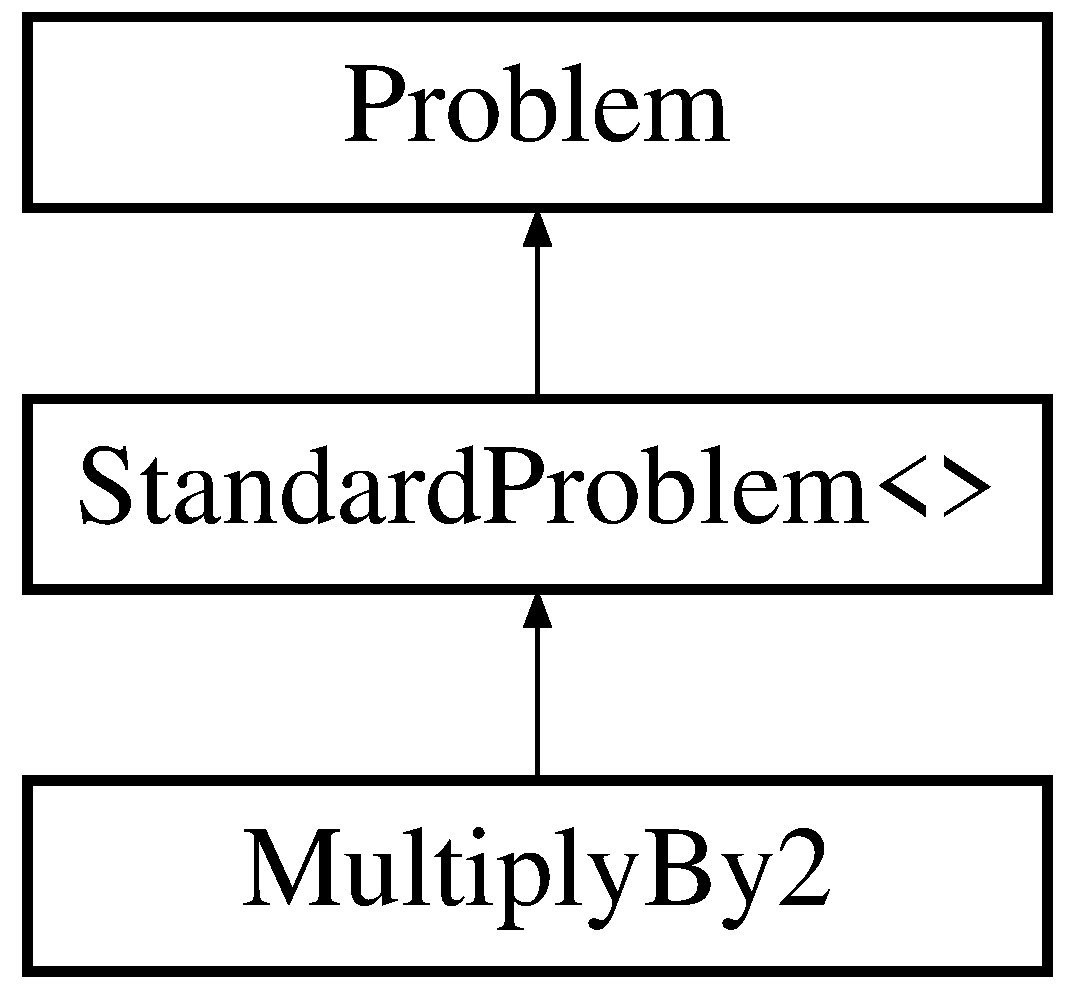
\includegraphics[height=3.000000cm]{class_multiply_by2}
\end{center}
\end{figure}
\subsection*{Metody publiczne}
\begin{DoxyCompactItemize}
\item 
void \hyperlink{class_multiply_by2_a77fc7fe07db4a9b52997320ff118d00f}{compute} ()
\begin{DoxyCompactList}\small\item\em Przemnaża tablicę wejściową przez 2. \end{DoxyCompactList}\item 
\hyperlink{class_multiply_by2_aace0e29d2ff880018a25a0e445e35a71}{$\sim$\-Multiply\-By2} ()=default
\end{DoxyCompactItemize}
\subsection*{Dodatkowe Dziedziczone Składowe}


\subsection{Opis szczegółowy}
Klasa reprezentuje algorytm mnożenia tablicy przez 2. 

\subsection{Dokumentacja konstruktora i destruktora}
\hypertarget{class_multiply_by2_aace0e29d2ff880018a25a0e445e35a71}{\index{Multiply\-By2@{Multiply\-By2}!$\sim$\-Multiply\-By2@{$\sim$\-Multiply\-By2}}
\index{$\sim$\-Multiply\-By2@{$\sim$\-Multiply\-By2}!MultiplyBy2@{Multiply\-By2}}
\subsubsection[{$\sim$\-Multiply\-By2}]{\setlength{\rightskip}{0pt plus 5cm}Multiply\-By2\-::$\sim$\-Multiply\-By2 (
\begin{DoxyParamCaption}
{}
\end{DoxyParamCaption}
)\hspace{0.3cm}{\ttfamily [default]}}}\label{class_multiply_by2_aace0e29d2ff880018a25a0e445e35a71}


\subsection{Dokumentacja funkcji składowych}
\hypertarget{class_multiply_by2_a77fc7fe07db4a9b52997320ff118d00f}{\index{Multiply\-By2@{Multiply\-By2}!compute@{compute}}
\index{compute@{compute}!MultiplyBy2@{Multiply\-By2}}
\subsubsection[{compute}]{\setlength{\rightskip}{0pt plus 5cm}void Multiply\-By2\-::compute (
\begin{DoxyParamCaption}
{}
\end{DoxyParamCaption}
)\hspace{0.3cm}{\ttfamily [virtual]}}}\label{class_multiply_by2_a77fc7fe07db4a9b52997320ff118d00f}


Przemnaża tablicę wejściową przez 2. 

Metoda wymnaża każdy element przez dwa i zapisuje wynik do tablicy wyjściowej 

Implementuje \hyperlink{class_standard_problem_ad9d90f5c981806bed7c6b4a08abb0384}{Standard\-Problem$<$$>$}.



Dokumentacja dla tej klasy została wygenerowana z plików\-:\begin{DoxyCompactItemize}
\item 
/home/mochman/\-Politechnika/\-P\-A\-M\-S\-I/benchmark-\/multiply-\/by-\/2/prj/inc/\hyperlink{_multiply_by2_8hpp}{Multiply\-By2.\-hpp}\item 
/home/mochman/\-Politechnika/\-P\-A\-M\-S\-I/benchmark-\/multiply-\/by-\/2/prj/src/\hyperlink{_multiply_by2_8cpp}{Multiply\-By2.\-cpp}\end{DoxyCompactItemize}

\hypertarget{class_problem}{\section{Dokumentacja klasy Problem}
\label{class_problem}\index{Problem@{Problem}}
}


Abstrakcyjna klasa reprezentująca problem algorytmiczny.  




{\ttfamily \#include $<$Problem.\-hpp$>$}

Diagram dziedziczenia dla Problem\begin{figure}[H]
\begin{center}
\leavevmode
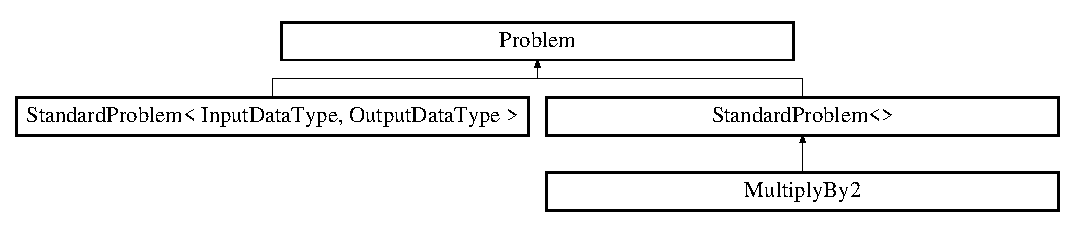
\includegraphics[height=2.608696cm]{class_problem}
\end{center}
\end{figure}
\subsection*{Metody publiczne}
\begin{DoxyCompactItemize}
\item 
virtual void \hyperlink{class_problem_a8e3f5755480a44a5dfe767b5429572c9}{read\-In\-Data} (std\-::istream \&is=std\-::cin)=0
\begin{DoxyCompactList}\small\item\em Wczytuje dane wejściowe algorytmu. \end{DoxyCompactList}\item 
virtual void \hyperlink{class_problem_af92be524acb6f1d6b484eff1fce07d2c}{read\-Out\-Data} (std\-::istream \&is=std\-::cin)=0
\begin{DoxyCompactList}\small\item\em Wczytuje poprawne dane wyjściowe algorytmu. \end{DoxyCompactList}\item 
virtual bool \hyperlink{class_problem_a55aef8681a2282a431abb77039cd01c1}{is\-Correct} () const =0
\begin{DoxyCompactList}\small\item\em Sprawdza czy wynik algorytmu jest poprawny. \end{DoxyCompactList}\item 
virtual void \hyperlink{class_problem_a278fa7a764e308758dbf9c07757ef037}{compute} ()=0
\begin{DoxyCompactList}\small\item\em Rozpoczyna pracę algorytmu. \end{DoxyCompactList}\item 
virtual unsigned int \hyperlink{class_problem_a938aceef78b28c64c03616a3fa619ec0}{problem\-Size} () const =0
\begin{DoxyCompactList}\small\item\em Pozwala pobrać rozmiar problemu. \end{DoxyCompactList}\item 
virtual void \hyperlink{class_problem_aa67aec5ea247cc9e6616a71345399a08}{problem\-Size} (unsigned int size)=0
\begin{DoxyCompactList}\small\item\em Pozwala ustawić rozmiar problemu. \end{DoxyCompactList}\item 
virtual void \hyperlink{class_problem_ad44a9ce61243b8f5c396795262990b82}{clear\-Data} ()=0
\begin{DoxyCompactList}\small\item\em Usuwa wszystkie dane. \end{DoxyCompactList}\item 
virtual \hyperlink{class_problem_ab31e378c1a54e149c8c6df5f6a534cad}{$\sim$\-Problem} ()=default
\end{DoxyCompactItemize}


\subsection{Opis szczegółowy}
Abstrakcyjna klasa reprezentująca problem algorytmiczny. 

Definiuje interfejs podstawowych operacji dla problemu tzn. wczytanie danych, przeprowadzenie obliczeń, sprawdzenie poprawności algorytmu 

\subsection{Dokumentacja konstruktora i destruktora}
\hypertarget{class_problem_ab31e378c1a54e149c8c6df5f6a534cad}{\index{Problem@{Problem}!$\sim$\-Problem@{$\sim$\-Problem}}
\index{$\sim$\-Problem@{$\sim$\-Problem}!Problem@{Problem}}
\subsubsection[{$\sim$\-Problem}]{\setlength{\rightskip}{0pt plus 5cm}virtual Problem\-::$\sim$\-Problem (
\begin{DoxyParamCaption}
{}
\end{DoxyParamCaption}
)\hspace{0.3cm}{\ttfamily [virtual]}, {\ttfamily [default]}}}\label{class_problem_ab31e378c1a54e149c8c6df5f6a534cad}


\subsection{Dokumentacja funkcji składowych}
\hypertarget{class_problem_ad44a9ce61243b8f5c396795262990b82}{\index{Problem@{Problem}!clear\-Data@{clear\-Data}}
\index{clear\-Data@{clear\-Data}!Problem@{Problem}}
\subsubsection[{clear\-Data}]{\setlength{\rightskip}{0pt plus 5cm}virtual void Problem\-::clear\-Data (
\begin{DoxyParamCaption}
{}
\end{DoxyParamCaption}
)\hspace{0.3cm}{\ttfamily [pure virtual]}}}\label{class_problem_ad44a9ce61243b8f5c396795262990b82}


Usuwa wszystkie dane. 

Pozbywa się z pamięci wszyskich danych wejsciowych, poprawnych wyjsciowych itp 

Implementowany w \hyperlink{class_standard_problem_a18639f20294c49814faf32a04f1317fa}{Standard\-Problem$<$ Input\-Data\-Type, Output\-Data\-Type $>$} i \hyperlink{class_standard_problem_a18639f20294c49814faf32a04f1317fa}{Standard\-Problem$<$$>$}.

\hypertarget{class_problem_a278fa7a764e308758dbf9c07757ef037}{\index{Problem@{Problem}!compute@{compute}}
\index{compute@{compute}!Problem@{Problem}}
\subsubsection[{compute}]{\setlength{\rightskip}{0pt plus 5cm}virtual void Problem\-::compute (
\begin{DoxyParamCaption}
{}
\end{DoxyParamCaption}
)\hspace{0.3cm}{\ttfamily [pure virtual]}}}\label{class_problem_a278fa7a764e308758dbf9c07757ef037}


Rozpoczyna pracę algorytmu. 



Implementowany w \hyperlink{class_standard_problem_ad9d90f5c981806bed7c6b4a08abb0384}{Standard\-Problem$<$ Input\-Data\-Type, Output\-Data\-Type $>$}, \hyperlink{class_standard_problem_ad9d90f5c981806bed7c6b4a08abb0384}{Standard\-Problem$<$$>$} i \hyperlink{class_multiply_by2_a77fc7fe07db4a9b52997320ff118d00f}{Multiply\-By2}.

\hypertarget{class_problem_a55aef8681a2282a431abb77039cd01c1}{\index{Problem@{Problem}!is\-Correct@{is\-Correct}}
\index{is\-Correct@{is\-Correct}!Problem@{Problem}}
\subsubsection[{is\-Correct}]{\setlength{\rightskip}{0pt plus 5cm}virtual bool Problem\-::is\-Correct (
\begin{DoxyParamCaption}
{}
\end{DoxyParamCaption}
) const\hspace{0.3cm}{\ttfamily [pure virtual]}}}\label{class_problem_a55aef8681a2282a431abb77039cd01c1}


Sprawdza czy wynik algorytmu jest poprawny. 

Dokonuje porównania wczytanych poprawnych danych z wynikiem algorytmu 

Implementowany w \hyperlink{class_standard_problem_aeab390b5968292a6bcb95d13d98bc62e}{Standard\-Problem$<$ Input\-Data\-Type, Output\-Data\-Type $>$} i \hyperlink{class_standard_problem_aeab390b5968292a6bcb95d13d98bc62e}{Standard\-Problem$<$$>$}.

\hypertarget{class_problem_a938aceef78b28c64c03616a3fa619ec0}{\index{Problem@{Problem}!problem\-Size@{problem\-Size}}
\index{problem\-Size@{problem\-Size}!Problem@{Problem}}
\subsubsection[{problem\-Size}]{\setlength{\rightskip}{0pt plus 5cm}virtual unsigned int Problem\-::problem\-Size (
\begin{DoxyParamCaption}
{}
\end{DoxyParamCaption}
) const\hspace{0.3cm}{\ttfamily [pure virtual]}}}\label{class_problem_a938aceef78b28c64c03616a3fa619ec0}


Pozwala pobrać rozmiar problemu. 



Implementowany w \hyperlink{class_standard_problem_a5a17f86a21c915ae373a273a01be91ac}{Standard\-Problem$<$ Input\-Data\-Type, Output\-Data\-Type $>$} i \hyperlink{class_standard_problem_a5a17f86a21c915ae373a273a01be91ac}{Standard\-Problem$<$$>$}.

\hypertarget{class_problem_aa67aec5ea247cc9e6616a71345399a08}{\index{Problem@{Problem}!problem\-Size@{problem\-Size}}
\index{problem\-Size@{problem\-Size}!Problem@{Problem}}
\subsubsection[{problem\-Size}]{\setlength{\rightskip}{0pt plus 5cm}virtual void Problem\-::problem\-Size (
\begin{DoxyParamCaption}
\item[{unsigned int}]{size}
\end{DoxyParamCaption}
)\hspace{0.3cm}{\ttfamily [pure virtual]}}}\label{class_problem_aa67aec5ea247cc9e6616a71345399a08}


Pozwala ustawić rozmiar problemu. 



Implementowany w \hyperlink{class_standard_problem_acddecc170b1e6e1c662df258ebfd5881}{Standard\-Problem$<$ Input\-Data\-Type, Output\-Data\-Type $>$} i \hyperlink{class_standard_problem_acddecc170b1e6e1c662df258ebfd5881}{Standard\-Problem$<$$>$}.

\hypertarget{class_problem_a8e3f5755480a44a5dfe767b5429572c9}{\index{Problem@{Problem}!read\-In\-Data@{read\-In\-Data}}
\index{read\-In\-Data@{read\-In\-Data}!Problem@{Problem}}
\subsubsection[{read\-In\-Data}]{\setlength{\rightskip}{0pt plus 5cm}virtual void Problem\-::read\-In\-Data (
\begin{DoxyParamCaption}
\item[{std\-::istream \&}]{is = {\ttfamily std\-:\-:cin}}
\end{DoxyParamCaption}
)\hspace{0.3cm}{\ttfamily [pure virtual]}}}\label{class_problem_a8e3f5755480a44a5dfe767b5429572c9}


Wczytuje dane wejściowe algorytmu. 


\begin{DoxyParams}{Parametry}
{\em is} & -\/ strumień z którego mają zostać wczytane dane \\
\hline
\end{DoxyParams}


Implementowany w \hyperlink{class_standard_problem_aaaf63ba0accbe5a4d6182fef2ccc448b}{Standard\-Problem$<$ Input\-Data\-Type, Output\-Data\-Type $>$} i \hyperlink{class_standard_problem_aaaf63ba0accbe5a4d6182fef2ccc448b}{Standard\-Problem$<$$>$}.

\hypertarget{class_problem_af92be524acb6f1d6b484eff1fce07d2c}{\index{Problem@{Problem}!read\-Out\-Data@{read\-Out\-Data}}
\index{read\-Out\-Data@{read\-Out\-Data}!Problem@{Problem}}
\subsubsection[{read\-Out\-Data}]{\setlength{\rightskip}{0pt plus 5cm}virtual void Problem\-::read\-Out\-Data (
\begin{DoxyParamCaption}
\item[{std\-::istream \&}]{is = {\ttfamily std\-:\-:cin}}
\end{DoxyParamCaption}
)\hspace{0.3cm}{\ttfamily [pure virtual]}}}\label{class_problem_af92be524acb6f1d6b484eff1fce07d2c}


Wczytuje poprawne dane wyjściowe algorytmu. 


\begin{DoxyParams}{Parametry}
{\em is} & -\/ strumień z którego mają zostać wczytane dane \\
\hline
\end{DoxyParams}


Implementowany w \hyperlink{class_standard_problem_a57d12a8e60de6af15273df44527a0769}{Standard\-Problem$<$ Input\-Data\-Type, Output\-Data\-Type $>$} i \hyperlink{class_standard_problem_a57d12a8e60de6af15273df44527a0769}{Standard\-Problem$<$$>$}.



Dokumentacja dla tej klasy została wygenerowana z pliku\-:\begin{DoxyCompactItemize}
\item 
/home/mochman/\-Politechnika/\-P\-A\-M\-S\-I/benchmark-\/multiply-\/by-\/2/prj/inc/\hyperlink{_problem_8hpp}{Problem.\-hpp}\end{DoxyCompactItemize}

\hypertarget{class_standard_problem}{\section{Dokumentacja szablonu klasy Standard\-Problem$<$ Input\-Data\-Type, Output\-Data\-Type $>$}
\label{class_standard_problem}\index{Standard\-Problem$<$ Input\-Data\-Type, Output\-Data\-Type $>$@{Standard\-Problem$<$ Input\-Data\-Type, Output\-Data\-Type $>$}}
}


Klasa definiuje standardowy problem algorytmiczny.  




{\ttfamily \#include $<$Standard\-Problem.\-hpp$>$}

Diagram dziedziczenia dla Standard\-Problem$<$ Input\-Data\-Type, Output\-Data\-Type $>$\begin{figure}[H]
\begin{center}
\leavevmode
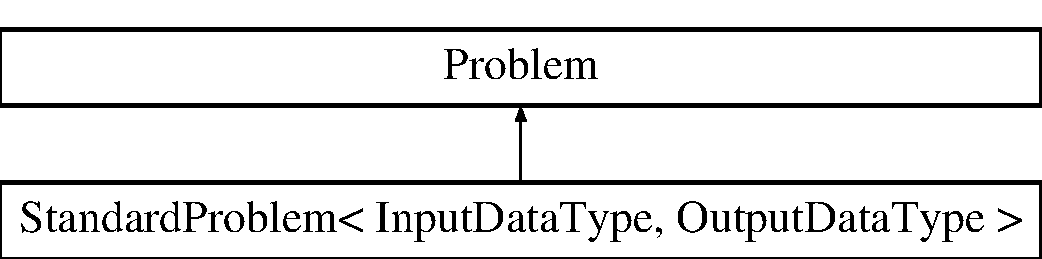
\includegraphics[height=2.000000cm]{class_standard_problem}
\end{center}
\end{figure}
\subsection*{Metody publiczne}
\begin{DoxyCompactItemize}
\item 
virtual void \hyperlink{class_standard_problem_aaaf63ba0accbe5a4d6182fef2ccc448b}{read\-In\-Data} (std\-::istream \&is=std\-::cin)
\begin{DoxyCompactList}\small\item\em Patrz \hyperlink{class_problem_a8e3f5755480a44a5dfe767b5429572c9}{Problem\-::read\-In\-Data}. \end{DoxyCompactList}\item 
virtual void \hyperlink{class_standard_problem_a57d12a8e60de6af15273df44527a0769}{read\-Out\-Data} (std\-::istream \&is=std\-::cin)
\begin{DoxyCompactList}\small\item\em Patrz \hyperlink{class_problem_af92be524acb6f1d6b484eff1fce07d2c}{Problem\-::read\-Out\-Data}. \end{DoxyCompactList}\item 
virtual bool \hyperlink{class_standard_problem_aeab390b5968292a6bcb95d13d98bc62e}{is\-Correct} () const 
\begin{DoxyCompactList}\small\item\em Patrz \hyperlink{class_problem_a55aef8681a2282a431abb77039cd01c1}{Problem\-::is\-Correct}. \end{DoxyCompactList}\item 
virtual void \hyperlink{class_standard_problem_ad9d90f5c981806bed7c6b4a08abb0384}{compute} ()=0
\begin{DoxyCompactList}\small\item\em Patrz \hyperlink{class_problem_a278fa7a764e308758dbf9c07757ef037}{Problem\-::compute}. \end{DoxyCompactList}\item 
virtual unsigned int \hyperlink{class_standard_problem_a5a17f86a21c915ae373a273a01be91ac}{problem\-Size} () const 
\begin{DoxyCompactList}\small\item\em Patrz \hyperlink{class_problem_a938aceef78b28c64c03616a3fa619ec0}{Problem\-::problem\-Size}. \end{DoxyCompactList}\item 
virtual void \hyperlink{class_standard_problem_acddecc170b1e6e1c662df258ebfd5881}{problem\-Size} (unsigned int size)
\begin{DoxyCompactList}\small\item\em Patrz \hyperlink{class_problem_aa67aec5ea247cc9e6616a71345399a08}{Problem\-::problem\-Size(unsigned int)} \end{DoxyCompactList}\item 
virtual void \hyperlink{class_standard_problem_a18639f20294c49814faf32a04f1317fa}{clear\-Data} ()
\begin{DoxyCompactList}\small\item\em Usuwa wszystkie dane. \end{DoxyCompactList}\end{DoxyCompactItemize}
\subsection*{Atrybuty chronione}
\begin{DoxyCompactItemize}
\item 
std\-::vector$<$ Input\-Data\-Type $>$ \hyperlink{class_standard_problem_ad1d5f039cd59372664a18ee57485252a}{m\-\_\-input\-Data}
\begin{DoxyCompactList}\small\item\em Wektor przechowujący dane wejściowe. \end{DoxyCompactList}\item 
std\-::vector$<$ Output\-Data\-Type $>$ \hyperlink{class_standard_problem_a2ca81280f88e1d8091cacceae8f2e073}{m\-\_\-output\-Data}
\begin{DoxyCompactList}\small\item\em Wektor przechowujący dane wyjściowe. \end{DoxyCompactList}\item 
std\-::vector$<$ Output\-Data\-Type $>$ \hyperlink{class_standard_problem_a7b736a0a91726c54363cedc43c80fbd2}{m\-\_\-correct\-Output\-Data}
\begin{DoxyCompactList}\small\item\em Wektor przechowujący poprawne dane wyjściowe. \end{DoxyCompactList}\end{DoxyCompactItemize}
\subsection*{Atrybuty prywatne}
\begin{DoxyCompactItemize}
\item 
unsigned int \hyperlink{class_standard_problem_ae8fc195a5e90d5cf0dd6c0417654741a}{m\-\_\-problem\-Size}
\begin{DoxyCompactList}\small\item\em Pole przechowujące rozmiar problemu. \end{DoxyCompactList}\end{DoxyCompactItemize}


\subsection{Opis szczegółowy}
\subsubsection*{template$<$typename Input\-Data\-Type = double, typename Output\-Data\-Type = double$>$class Standard\-Problem$<$ Input\-Data\-Type, Output\-Data\-Type $>$}

Klasa definiuje standardowy problem algorytmiczny. 

Poprzez standardowy problem algorytmiczny rozumiem problem, w którym wczytuje się rozmiar problemu a następnie tablicę tego samego typu. Wynikiem jest zbiór liczb tego samego typu o tej samej liczności Przykładem może być np. mnożenie tablicy przez stałą, sortowanie itp. 

\subsection{Dokumentacja funkcji składowych}
\hypertarget{class_standard_problem_a18639f20294c49814faf32a04f1317fa}{\index{Standard\-Problem@{Standard\-Problem}!clear\-Data@{clear\-Data}}
\index{clear\-Data@{clear\-Data}!StandardProblem@{Standard\-Problem}}
\subsubsection[{clear\-Data}]{\setlength{\rightskip}{0pt plus 5cm}template$<$typename Input\-Data\-Type , typename Output\-Data\-Type $>$ void {\bf Standard\-Problem}$<$ Input\-Data\-Type, Output\-Data\-Type $>$\-::clear\-Data (
\begin{DoxyParamCaption}
{}
\end{DoxyParamCaption}
)\hspace{0.3cm}{\ttfamily [virtual]}}}\label{class_standard_problem_a18639f20294c49814faf32a04f1317fa}


Usuwa wszystkie dane. 

Pozbywa się z pamięci wszyskich danych wejsciowych, poprawnych wyjsciowych itp 

Implementuje \hyperlink{class_problem_ad44a9ce61243b8f5c396795262990b82}{Problem}.

\hypertarget{class_standard_problem_ad9d90f5c981806bed7c6b4a08abb0384}{\index{Standard\-Problem@{Standard\-Problem}!compute@{compute}}
\index{compute@{compute}!StandardProblem@{Standard\-Problem}}
\subsubsection[{compute}]{\setlength{\rightskip}{0pt plus 5cm}template$<$typename Input\-Data\-Type = double, typename Output\-Data\-Type = double$>$ virtual void {\bf Standard\-Problem}$<$ Input\-Data\-Type, Output\-Data\-Type $>$\-::compute (
\begin{DoxyParamCaption}
{}
\end{DoxyParamCaption}
)\hspace{0.3cm}{\ttfamily [pure virtual]}}}\label{class_standard_problem_ad9d90f5c981806bed7c6b4a08abb0384}


Patrz \hyperlink{class_problem_a278fa7a764e308758dbf9c07757ef037}{Problem\-::compute}. 



Implementuje \hyperlink{class_problem_a278fa7a764e308758dbf9c07757ef037}{Problem}.



Implementowany w \hyperlink{class_multiply_by2_a77fc7fe07db4a9b52997320ff118d00f}{Multiply\-By2}.

\hypertarget{class_standard_problem_aeab390b5968292a6bcb95d13d98bc62e}{\index{Standard\-Problem@{Standard\-Problem}!is\-Correct@{is\-Correct}}
\index{is\-Correct@{is\-Correct}!StandardProblem@{Standard\-Problem}}
\subsubsection[{is\-Correct}]{\setlength{\rightskip}{0pt plus 5cm}template$<$typename Input\-Data\-Type , typename Output\-Data\-Type $>$ bool {\bf Standard\-Problem}$<$ Input\-Data\-Type, Output\-Data\-Type $>$\-::is\-Correct (
\begin{DoxyParamCaption}
{}
\end{DoxyParamCaption}
) const\hspace{0.3cm}{\ttfamily [virtual]}}}\label{class_standard_problem_aeab390b5968292a6bcb95d13d98bc62e}


Patrz \hyperlink{class_problem_a55aef8681a2282a431abb77039cd01c1}{Problem\-::is\-Correct}. 



Implementuje \hyperlink{class_problem_a55aef8681a2282a431abb77039cd01c1}{Problem}.

\hypertarget{class_standard_problem_a5a17f86a21c915ae373a273a01be91ac}{\index{Standard\-Problem@{Standard\-Problem}!problem\-Size@{problem\-Size}}
\index{problem\-Size@{problem\-Size}!StandardProblem@{Standard\-Problem}}
\subsubsection[{problem\-Size}]{\setlength{\rightskip}{0pt plus 5cm}template$<$typename Input\-Data\-Type = double, typename Output\-Data\-Type = double$>$ virtual unsigned int {\bf Standard\-Problem}$<$ Input\-Data\-Type, Output\-Data\-Type $>$\-::problem\-Size (
\begin{DoxyParamCaption}
{}
\end{DoxyParamCaption}
) const\hspace{0.3cm}{\ttfamily [inline]}, {\ttfamily [virtual]}}}\label{class_standard_problem_a5a17f86a21c915ae373a273a01be91ac}


Patrz \hyperlink{class_problem_a938aceef78b28c64c03616a3fa619ec0}{Problem\-::problem\-Size}. 



Implementuje \hyperlink{class_problem_a938aceef78b28c64c03616a3fa619ec0}{Problem}.

\hypertarget{class_standard_problem_acddecc170b1e6e1c662df258ebfd5881}{\index{Standard\-Problem@{Standard\-Problem}!problem\-Size@{problem\-Size}}
\index{problem\-Size@{problem\-Size}!StandardProblem@{Standard\-Problem}}
\subsubsection[{problem\-Size}]{\setlength{\rightskip}{0pt plus 5cm}template$<$typename Input\-Data\-Type = double, typename Output\-Data\-Type = double$>$ virtual void {\bf Standard\-Problem}$<$ Input\-Data\-Type, Output\-Data\-Type $>$\-::problem\-Size (
\begin{DoxyParamCaption}
\item[{unsigned int}]{size}
\end{DoxyParamCaption}
)\hspace{0.3cm}{\ttfamily [inline]}, {\ttfamily [virtual]}}}\label{class_standard_problem_acddecc170b1e6e1c662df258ebfd5881}


Patrz \hyperlink{class_problem_aa67aec5ea247cc9e6616a71345399a08}{Problem\-::problem\-Size(unsigned int)} 

Dodatkowo zmiana powoduje wyczyszczenie wszystkich danych oraz rezerwację pamięci o odpowiedniej wielkości 

Implementuje \hyperlink{class_problem_aa67aec5ea247cc9e6616a71345399a08}{Problem}.

\hypertarget{class_standard_problem_aaaf63ba0accbe5a4d6182fef2ccc448b}{\index{Standard\-Problem@{Standard\-Problem}!read\-In\-Data@{read\-In\-Data}}
\index{read\-In\-Data@{read\-In\-Data}!StandardProblem@{Standard\-Problem}}
\subsubsection[{read\-In\-Data}]{\setlength{\rightskip}{0pt plus 5cm}template$<$typename Input\-Data\-Type , typename Output\-Data\-Type $>$ void {\bf Standard\-Problem}$<$ Input\-Data\-Type, Output\-Data\-Type $>$\-::read\-In\-Data (
\begin{DoxyParamCaption}
\item[{std\-::istream \&}]{is = {\ttfamily std\-:\-:cin}}
\end{DoxyParamCaption}
)\hspace{0.3cm}{\ttfamily [virtual]}}}\label{class_standard_problem_aaaf63ba0accbe5a4d6182fef2ccc448b}


Patrz \hyperlink{class_problem_a8e3f5755480a44a5dfe767b5429572c9}{Problem\-::read\-In\-Data}. 



Implementuje \hyperlink{class_problem_a8e3f5755480a44a5dfe767b5429572c9}{Problem}.

\hypertarget{class_standard_problem_a57d12a8e60de6af15273df44527a0769}{\index{Standard\-Problem@{Standard\-Problem}!read\-Out\-Data@{read\-Out\-Data}}
\index{read\-Out\-Data@{read\-Out\-Data}!StandardProblem@{Standard\-Problem}}
\subsubsection[{read\-Out\-Data}]{\setlength{\rightskip}{0pt plus 5cm}template$<$typename Input\-Data\-Type , typename Output\-Data\-Type $>$ void {\bf Standard\-Problem}$<$ Input\-Data\-Type, Output\-Data\-Type $>$\-::read\-Out\-Data (
\begin{DoxyParamCaption}
\item[{std\-::istream \&}]{is = {\ttfamily std\-:\-:cin}}
\end{DoxyParamCaption}
)\hspace{0.3cm}{\ttfamily [virtual]}}}\label{class_standard_problem_a57d12a8e60de6af15273df44527a0769}


Patrz \hyperlink{class_problem_af92be524acb6f1d6b484eff1fce07d2c}{Problem\-::read\-Out\-Data}. 



Implementuje \hyperlink{class_problem_af92be524acb6f1d6b484eff1fce07d2c}{Problem}.



\subsection{Dokumentacja atrybutów składowych}
\hypertarget{class_standard_problem_a7b736a0a91726c54363cedc43c80fbd2}{\index{Standard\-Problem@{Standard\-Problem}!m\-\_\-correct\-Output\-Data@{m\-\_\-correct\-Output\-Data}}
\index{m\-\_\-correct\-Output\-Data@{m\-\_\-correct\-Output\-Data}!StandardProblem@{Standard\-Problem}}
\subsubsection[{m\-\_\-correct\-Output\-Data}]{\setlength{\rightskip}{0pt plus 5cm}template$<$typename Input\-Data\-Type = double, typename Output\-Data\-Type = double$>$ std\-::vector$<$Output\-Data\-Type$>$ {\bf Standard\-Problem}$<$ Input\-Data\-Type, Output\-Data\-Type $>$\-::m\-\_\-correct\-Output\-Data\hspace{0.3cm}{\ttfamily [protected]}}}\label{class_standard_problem_a7b736a0a91726c54363cedc43c80fbd2}


Wektor przechowujący poprawne dane wyjściowe. 

Z tymi dany jest porównywane wyjście algorytmu i sprawdzana poprawność algorytmu. \hypertarget{class_standard_problem_ad1d5f039cd59372664a18ee57485252a}{\index{Standard\-Problem@{Standard\-Problem}!m\-\_\-input\-Data@{m\-\_\-input\-Data}}
\index{m\-\_\-input\-Data@{m\-\_\-input\-Data}!StandardProblem@{Standard\-Problem}}
\subsubsection[{m\-\_\-input\-Data}]{\setlength{\rightskip}{0pt plus 5cm}template$<$typename Input\-Data\-Type = double, typename Output\-Data\-Type = double$>$ std\-::vector$<$Input\-Data\-Type$>$ {\bf Standard\-Problem}$<$ Input\-Data\-Type, Output\-Data\-Type $>$\-::m\-\_\-input\-Data\hspace{0.3cm}{\ttfamily [protected]}}}\label{class_standard_problem_ad1d5f039cd59372664a18ee57485252a}


Wektor przechowujący dane wejściowe. 

\hypertarget{class_standard_problem_a2ca81280f88e1d8091cacceae8f2e073}{\index{Standard\-Problem@{Standard\-Problem}!m\-\_\-output\-Data@{m\-\_\-output\-Data}}
\index{m\-\_\-output\-Data@{m\-\_\-output\-Data}!StandardProblem@{Standard\-Problem}}
\subsubsection[{m\-\_\-output\-Data}]{\setlength{\rightskip}{0pt plus 5cm}template$<$typename Input\-Data\-Type = double, typename Output\-Data\-Type = double$>$ std\-::vector$<$Output\-Data\-Type$>$ {\bf Standard\-Problem}$<$ Input\-Data\-Type, Output\-Data\-Type $>$\-::m\-\_\-output\-Data\hspace{0.3cm}{\ttfamily [protected]}}}\label{class_standard_problem_a2ca81280f88e1d8091cacceae8f2e073}


Wektor przechowujący dane wyjściowe. 

Są to dane wygenerowane poprzez metodę \hyperlink{class_standard_problem_ad9d90f5c981806bed7c6b4a08abb0384}{compute()} \hypertarget{class_standard_problem_ae8fc195a5e90d5cf0dd6c0417654741a}{\index{Standard\-Problem@{Standard\-Problem}!m\-\_\-problem\-Size@{m\-\_\-problem\-Size}}
\index{m\-\_\-problem\-Size@{m\-\_\-problem\-Size}!StandardProblem@{Standard\-Problem}}
\subsubsection[{m\-\_\-problem\-Size}]{\setlength{\rightskip}{0pt plus 5cm}template$<$typename Input\-Data\-Type = double, typename Output\-Data\-Type = double$>$ unsigned int {\bf Standard\-Problem}$<$ Input\-Data\-Type, Output\-Data\-Type $>$\-::m\-\_\-problem\-Size\hspace{0.3cm}{\ttfamily [private]}}}\label{class_standard_problem_ae8fc195a5e90d5cf0dd6c0417654741a}


Pole przechowujące rozmiar problemu. 



Dokumentacja dla tej klasy została wygenerowana z pliku\-:\begin{DoxyCompactItemize}
\item 
/home/mochman/\-Politechnika/\-P\-A\-M\-S\-I/benchmark-\/multiply-\/by-\/2/prj/inc/\hyperlink{_standard_problem_8hpp}{Standard\-Problem.\-hpp}\end{DoxyCompactItemize}

\hypertarget{class_timer}{\section{Dokumentacja klasy Timer}
\label{class_timer}\index{Timer@{Timer}}
}


Klasa mierząca długość interwału czasu.  




{\ttfamily \#include $<$Timer.\-hpp$>$}

\subsection*{Metody publiczne}
\begin{DoxyCompactItemize}
\item 
double \hyperlink{class_timer_a2dd502fa5a0d6827da5578e292d96942}{ns\-Interval} () const 
\begin{DoxyCompactList}\small\item\em Oblicza długość odcinka czasu w nanosekundach. \end{DoxyCompactList}\item 
double \hyperlink{class_timer_a124742f864cf5913b63807ff8b3a6c7a}{us\-Interval} () const 
\begin{DoxyCompactList}\small\item\em Oblicza długość odcinka czasu w mikrosekundach. \end{DoxyCompactList}\item 
double \hyperlink{class_timer_a82a672b3866241f01351b4581113aba3}{ms\-Interval} () const 
\begin{DoxyCompactList}\small\item\em Oblicza długość odcinka czasu w milisekundach. \end{DoxyCompactList}\item 
double \hyperlink{class_timer_acabb155ab43e81e2fc8c568d73d1d1d3}{s\-Interval} () const 
\begin{DoxyCompactList}\small\item\em Oblicza długość odcinka czasu w sekundach. \end{DoxyCompactList}\item 
void \hyperlink{class_timer_a3a8b5272198d029779dc9302a54305a8}{start} ()
\begin{DoxyCompactList}\small\item\em Zaczyna odmierzać czas. \end{DoxyCompactList}\item 
void \hyperlink{class_timer_a63f0eb44b27402196590a03781515dba}{stop} ()
\begin{DoxyCompactList}\small\item\em Kończy odmierzać czas. \end{DoxyCompactList}\end{DoxyCompactItemize}
\subsection*{Statyczne metody publiczne}
\begin{DoxyCompactItemize}
\item 
static double \hyperlink{class_timer_a65402ab97ec7d3009f3ee3edfa5b1db4}{precision} ()
\begin{DoxyCompactList}\small\item\em Zwraca precyzję zegara w sekundach. \end{DoxyCompactList}\end{DoxyCompactItemize}
\subsection*{Atrybuty prywatne}
\begin{DoxyCompactItemize}
\item 
std\-::chrono\-::high\-\_\-resolution\-\_\-clock\-::time\-\_\-point \hyperlink{class_timer_ac14f6ea6f71c3eef3c88780e009741c8}{m\-\_\-start}
\begin{DoxyCompactList}\small\item\em Przechowuje informacje o chwili od której odliczać czas. \end{DoxyCompactList}\item 
std\-::chrono\-::high\-\_\-resolution\-\_\-clock\-::time\-\_\-point \hyperlink{class_timer_a9aef0f9d32d37b36b843e60eb10d0644}{m\-\_\-end}
\begin{DoxyCompactList}\small\item\em Przechowuje informacje o chwili do której odliczać czas. \end{DoxyCompactList}\end{DoxyCompactItemize}


\subsection{Opis szczegółowy}
Klasa mierząca długość interwału czasu. 

Do funkcjonowania używa high\-\_\-resolution\-\_\-clock z z biblioteki standardowej C++. 

\subsection{Dokumentacja funkcji składowych}
\hypertarget{class_timer_a82a672b3866241f01351b4581113aba3}{\index{Timer@{Timer}!ms\-Interval@{ms\-Interval}}
\index{ms\-Interval@{ms\-Interval}!Timer@{Timer}}
\subsubsection[{ms\-Interval}]{\setlength{\rightskip}{0pt plus 5cm}double Timer\-::ms\-Interval (
\begin{DoxyParamCaption}
{}
\end{DoxyParamCaption}
) const}}\label{class_timer_a82a672b3866241f01351b4581113aba3}


Oblicza długość odcinka czasu w milisekundach. 

Jeśli nie została użyta metoda \hyperlink{class_timer_a3a8b5272198d029779dc9302a54305a8}{start()} to czas liczony jest od tzw epoch. Jeśli zostanie użyta metoda end() a \hyperlink{class_timer_a3a8b5272198d029779dc9302a54305a8}{start()} nie to pojawi się ujemny czas liczony od epoch \hypertarget{class_timer_a2dd502fa5a0d6827da5578e292d96942}{\index{Timer@{Timer}!ns\-Interval@{ns\-Interval}}
\index{ns\-Interval@{ns\-Interval}!Timer@{Timer}}
\subsubsection[{ns\-Interval}]{\setlength{\rightskip}{0pt plus 5cm}double Timer\-::ns\-Interval (
\begin{DoxyParamCaption}
{}
\end{DoxyParamCaption}
) const}}\label{class_timer_a2dd502fa5a0d6827da5578e292d96942}


Oblicza długość odcinka czasu w nanosekundach. 

Jeśli nie została użyta metoda \hyperlink{class_timer_a3a8b5272198d029779dc9302a54305a8}{start()} to czas liczony jest od tzw epoch. Jeśli zostanie użyta metoda end() a \hyperlink{class_timer_a3a8b5272198d029779dc9302a54305a8}{start()} nie to pojawi się ujemny czas liczony od epoch U\-W\-A\-G\-A! Nie na każdym systemie dokładność czasu jest tak duża! \hypertarget{class_timer_a65402ab97ec7d3009f3ee3edfa5b1db4}{\index{Timer@{Timer}!precision@{precision}}
\index{precision@{precision}!Timer@{Timer}}
\subsubsection[{precision}]{\setlength{\rightskip}{0pt plus 5cm}double Timer\-::precision (
\begin{DoxyParamCaption}
{}
\end{DoxyParamCaption}
)\hspace{0.3cm}{\ttfamily [static]}}}\label{class_timer_a65402ab97ec7d3009f3ee3edfa5b1db4}


Zwraca precyzję zegara w sekundach. 

\hypertarget{class_timer_acabb155ab43e81e2fc8c568d73d1d1d3}{\index{Timer@{Timer}!s\-Interval@{s\-Interval}}
\index{s\-Interval@{s\-Interval}!Timer@{Timer}}
\subsubsection[{s\-Interval}]{\setlength{\rightskip}{0pt plus 5cm}double Timer\-::s\-Interval (
\begin{DoxyParamCaption}
{}
\end{DoxyParamCaption}
) const}}\label{class_timer_acabb155ab43e81e2fc8c568d73d1d1d3}


Oblicza długość odcinka czasu w sekundach. 

Jeśli nie została użyta metoda \hyperlink{class_timer_a3a8b5272198d029779dc9302a54305a8}{start()} to czas liczony jest od tzw epoch. Jeśli zostanie użyta metoda end() a \hyperlink{class_timer_a3a8b5272198d029779dc9302a54305a8}{start()} nie to pojawi się ujemny czas liczony od epoch \hypertarget{class_timer_a3a8b5272198d029779dc9302a54305a8}{\index{Timer@{Timer}!start@{start}}
\index{start@{start}!Timer@{Timer}}
\subsubsection[{start}]{\setlength{\rightskip}{0pt plus 5cm}void Timer\-::start (
\begin{DoxyParamCaption}
{}
\end{DoxyParamCaption}
)\hspace{0.3cm}{\ttfamily [inline]}}}\label{class_timer_a3a8b5272198d029779dc9302a54305a8}


Zaczyna odmierzać czas. 

Metoda zapisuje do prywatnego pola aktualną chwilę, od której ma być liczony czas \hypertarget{class_timer_a63f0eb44b27402196590a03781515dba}{\index{Timer@{Timer}!stop@{stop}}
\index{stop@{stop}!Timer@{Timer}}
\subsubsection[{stop}]{\setlength{\rightskip}{0pt plus 5cm}void Timer\-::stop (
\begin{DoxyParamCaption}
{}
\end{DoxyParamCaption}
)\hspace{0.3cm}{\ttfamily [inline]}}}\label{class_timer_a63f0eb44b27402196590a03781515dba}


Kończy odmierzać czas. 

Metoda zapisuje do prywatnego pola aktualną chwilę, do której ma być liczony czas \hypertarget{class_timer_a124742f864cf5913b63807ff8b3a6c7a}{\index{Timer@{Timer}!us\-Interval@{us\-Interval}}
\index{us\-Interval@{us\-Interval}!Timer@{Timer}}
\subsubsection[{us\-Interval}]{\setlength{\rightskip}{0pt plus 5cm}double Timer\-::us\-Interval (
\begin{DoxyParamCaption}
{}
\end{DoxyParamCaption}
) const}}\label{class_timer_a124742f864cf5913b63807ff8b3a6c7a}


Oblicza długość odcinka czasu w mikrosekundach. 

Jeśli nie została użyta metoda \hyperlink{class_timer_a3a8b5272198d029779dc9302a54305a8}{start()} to czas liczony jest od tzw epoch. Jeśli zostanie użyta metoda end() a \hyperlink{class_timer_a3a8b5272198d029779dc9302a54305a8}{start()} nie to pojawi się ujemny czas liczony od epoch 

\subsection{Dokumentacja atrybutów składowych}
\hypertarget{class_timer_a9aef0f9d32d37b36b843e60eb10d0644}{\index{Timer@{Timer}!m\-\_\-end@{m\-\_\-end}}
\index{m\-\_\-end@{m\-\_\-end}!Timer@{Timer}}
\subsubsection[{m\-\_\-end}]{\setlength{\rightskip}{0pt plus 5cm}std\-::chrono\-::high\-\_\-resolution\-\_\-clock\-::time\-\_\-point Timer\-::m\-\_\-end\hspace{0.3cm}{\ttfamily [private]}}}\label{class_timer_a9aef0f9d32d37b36b843e60eb10d0644}


Przechowuje informacje o chwili do której odliczać czas. 

\hypertarget{class_timer_ac14f6ea6f71c3eef3c88780e009741c8}{\index{Timer@{Timer}!m\-\_\-start@{m\-\_\-start}}
\index{m\-\_\-start@{m\-\_\-start}!Timer@{Timer}}
\subsubsection[{m\-\_\-start}]{\setlength{\rightskip}{0pt plus 5cm}std\-::chrono\-::high\-\_\-resolution\-\_\-clock\-::time\-\_\-point Timer\-::m\-\_\-start\hspace{0.3cm}{\ttfamily [private]}}}\label{class_timer_ac14f6ea6f71c3eef3c88780e009741c8}


Przechowuje informacje o chwili od której odliczać czas. 



Dokumentacja dla tej klasy została wygenerowana z plików\-:\begin{DoxyCompactItemize}
\item 
/home/mochman/\-Politechnika/\-P\-A\-M\-S\-I/benchmark-\/multiply-\/by-\/2/prj/inc/\hyperlink{_timer_8hpp}{Timer.\-hpp}\item 
/home/mochman/\-Politechnika/\-P\-A\-M\-S\-I/benchmark-\/multiply-\/by-\/2/prj/src/\hyperlink{_timer_8cpp}{Timer.\-cpp}\end{DoxyCompactItemize}

\chapter{Dokumentacja plików}
\hypertarget{_main_page_8dox}{\section{Dokumentacja pliku /home/mochman/\-Politechnika/\-P\-A\-M\-S\-I/benchmark-\/multiply-\/by-\/2/prj/doxygen/\-Main\-Page.dox}
\label{_main_page_8dox}\index{/home/mochman/\-Politechnika/\-P\-A\-M\-S\-I/benchmark-\/multiply-\/by-\/2/prj/doxygen/\-Main\-Page.\-dox@{/home/mochman/\-Politechnika/\-P\-A\-M\-S\-I/benchmark-\/multiply-\/by-\/2/prj/doxygen/\-Main\-Page.\-dox}}
}

\hypertarget{_benchmark_8hpp}{\section{Dokumentacja pliku /home/mochman/\-Politechnika/\-P\-A\-M\-S\-I/benchmark-\/multiply-\/by-\/2/prj/inc/\-Benchmark.hpp}
\label{_benchmark_8hpp}\index{/home/mochman/\-Politechnika/\-P\-A\-M\-S\-I/benchmark-\/multiply-\/by-\/2/prj/inc/\-Benchmark.\-hpp@{/home/mochman/\-Politechnika/\-P\-A\-M\-S\-I/benchmark-\/multiply-\/by-\/2/prj/inc/\-Benchmark.\-hpp}}
}
{\ttfamily \#include $<$vector$>$}\\*
{\ttfamily \#include $<$iostream$>$}\\*
{\ttfamily \#include \char`\"{}Timer.\-hpp\char`\"{}}\\*
\subsection*{Komponenty}
\begin{DoxyCompactItemize}
\item 
struct \hyperlink{struct_benchmark_data}{Benchmark\-Data}
\begin{DoxyCompactList}\small\item\em Struktura przechowująca informacje o pojedynczym teście wydajności. \end{DoxyCompactList}\item 
class \hyperlink{class_benchmark}{Benchmark$<$ Problem\-Type $>$}
\begin{DoxyCompactList}\small\item\em Klasa pozwalająca na testowanie algorytmów. \end{DoxyCompactList}\end{DoxyCompactItemize}
\subsection*{Funkcje}
\begin{DoxyCompactItemize}
\item 
std\-::ostream \& \hyperlink{_benchmark_8hpp_aac3deb4ef9b981787d48e20b03ae2613}{operator$<$$<$} (std\-::ostream \&os, \hyperlink{struct_benchmark_data}{Benchmark\-Data} \&bench\-Data)
\begin{DoxyCompactList}\small\item\em Pozwala wyświetlić zawartość struktury. \end{DoxyCompactList}\end{DoxyCompactItemize}


\subsection{Dokumentacja funkcji}
\hypertarget{_benchmark_8hpp_aac3deb4ef9b981787d48e20b03ae2613}{\index{Benchmark.\-hpp@{Benchmark.\-hpp}!operator$<$$<$@{operator$<$$<$}}
\index{operator$<$$<$@{operator$<$$<$}!Benchmark.hpp@{Benchmark.\-hpp}}
\subsubsection[{operator$<$$<$}]{\setlength{\rightskip}{0pt plus 5cm}std\-::ostream \& operator$<$$<$ (
\begin{DoxyParamCaption}
\item[{std\-::ostream \&}]{os, }
\item[{{\bf Benchmark\-Data} \&}]{bench\-Data}
\end{DoxyParamCaption}
)}}\label{_benchmark_8hpp_aac3deb4ef9b981787d48e20b03ae2613}


Pozwala wyświetlić zawartość struktury. 

Format jest następujący\-: rozmiar problemu,numer porządkowy,czas wykonania 
\hypertarget{_multiply_by2_8hpp}{\section{Dokumentacja pliku /home/mochman/\-Politechnika/\-P\-A\-M\-S\-I/benchmark-\/multiply-\/by-\/2/prj/inc/\-Multiply\-By2.hpp}
\label{_multiply_by2_8hpp}\index{/home/mochman/\-Politechnika/\-P\-A\-M\-S\-I/benchmark-\/multiply-\/by-\/2/prj/inc/\-Multiply\-By2.\-hpp@{/home/mochman/\-Politechnika/\-P\-A\-M\-S\-I/benchmark-\/multiply-\/by-\/2/prj/inc/\-Multiply\-By2.\-hpp}}
}
{\ttfamily \#include \char`\"{}Standard\-Problem.\-hpp\char`\"{}}\\*
\subsection*{Komponenty}
\begin{DoxyCompactItemize}
\item 
class \hyperlink{class_multiply_by2}{Multiply\-By2}
\begin{DoxyCompactList}\small\item\em Klasa reprezentuje algorytm mnożenia tablicy przez 2. \end{DoxyCompactList}\end{DoxyCompactItemize}

\hypertarget{_problem_8hpp}{\section{Dokumentacja pliku /home/mochman/\-Politechnika/\-P\-A\-M\-S\-I/benchmark-\/multiply-\/by-\/2/prj/inc/\-Problem.hpp}
\label{_problem_8hpp}\index{/home/mochman/\-Politechnika/\-P\-A\-M\-S\-I/benchmark-\/multiply-\/by-\/2/prj/inc/\-Problem.\-hpp@{/home/mochman/\-Politechnika/\-P\-A\-M\-S\-I/benchmark-\/multiply-\/by-\/2/prj/inc/\-Problem.\-hpp}}
}
{\ttfamily \#include $<$iostream$>$}\\*
\subsection*{Komponenty}
\begin{DoxyCompactItemize}
\item 
class \hyperlink{class_problem}{Problem}
\begin{DoxyCompactList}\small\item\em Abstrakcyjna klasa reprezentująca problem algorytmiczny. \end{DoxyCompactList}\end{DoxyCompactItemize}

\hypertarget{_standard_problem_8hpp}{\section{Dokumentacja pliku /home/mochman/\-Politechnika/\-P\-A\-M\-S\-I/benchmark-\/multiply-\/by-\/2/prj/inc/\-Standard\-Problem.hpp}
\label{_standard_problem_8hpp}\index{/home/mochman/\-Politechnika/\-P\-A\-M\-S\-I/benchmark-\/multiply-\/by-\/2/prj/inc/\-Standard\-Problem.\-hpp@{/home/mochman/\-Politechnika/\-P\-A\-M\-S\-I/benchmark-\/multiply-\/by-\/2/prj/inc/\-Standard\-Problem.\-hpp}}
}
{\ttfamily \#include $<$vector$>$}\\*
{\ttfamily \#include \char`\"{}Problem.\-hpp\char`\"{}}\\*
\subsection*{Komponenty}
\begin{DoxyCompactItemize}
\item 
class \hyperlink{class_standard_problem}{Standard\-Problem$<$ Input\-Data\-Type, Output\-Data\-Type $>$}
\begin{DoxyCompactList}\small\item\em Klasa definiuje standardowy problem algorytmiczny. \end{DoxyCompactList}\end{DoxyCompactItemize}

\hypertarget{_timer_8hpp}{\section{Dokumentacja pliku /home/mochman/\-Politechnika/\-P\-A\-M\-S\-I/benchmark-\/multiply-\/by-\/2/prj/inc/\-Timer.hpp}
\label{_timer_8hpp}\index{/home/mochman/\-Politechnika/\-P\-A\-M\-S\-I/benchmark-\/multiply-\/by-\/2/prj/inc/\-Timer.\-hpp@{/home/mochman/\-Politechnika/\-P\-A\-M\-S\-I/benchmark-\/multiply-\/by-\/2/prj/inc/\-Timer.\-hpp}}
}
{\ttfamily \#include $<$chrono$>$}\\*
\subsection*{Komponenty}
\begin{DoxyCompactItemize}
\item 
class \hyperlink{class_timer}{Timer}
\begin{DoxyCompactList}\small\item\em Klasa mierząca długość interwału czasu. \end{DoxyCompactList}\end{DoxyCompactItemize}

\hypertarget{main_8cpp}{\section{Dokumentacja pliku /home/mochman/\-Politechnika/\-P\-A\-M\-S\-I/benchmark-\/multiply-\/by-\/2/prj/src/main.cpp}
\label{main_8cpp}\index{/home/mochman/\-Politechnika/\-P\-A\-M\-S\-I/benchmark-\/multiply-\/by-\/2/prj/src/main.\-cpp@{/home/mochman/\-Politechnika/\-P\-A\-M\-S\-I/benchmark-\/multiply-\/by-\/2/prj/src/main.\-cpp}}
}
{\ttfamily \#include \char`\"{}Benchmark.\-hpp\char`\"{}}\\*
{\ttfamily \#include \char`\"{}Multiply\-By2.\-hpp\char`\"{}}\\*
{\ttfamily \#include $<$string$>$}\\*
{\ttfamily \#include $<$fstream$>$}\\*
{\ttfamily \#include $<$thread$>$}\\*
\subsection*{Funkcje}
\begin{DoxyCompactItemize}
\item 
int \hyperlink{main_8cpp_a0ddf1224851353fc92bfbff6f499fa97}{main} (int argc, char $\ast$argv\mbox{[}$\,$\mbox{]})
\end{DoxyCompactItemize}


\subsection{Dokumentacja funkcji}
\hypertarget{main_8cpp_a0ddf1224851353fc92bfbff6f499fa97}{\index{main.\-cpp@{main.\-cpp}!main@{main}}
\index{main@{main}!main.cpp@{main.\-cpp}}
\subsubsection[{main}]{\setlength{\rightskip}{0pt plus 5cm}int main (
\begin{DoxyParamCaption}
\item[{int}]{argc, }
\item[{char $\ast$}]{argv\mbox{[}$\,$\mbox{]}}
\end{DoxyParamCaption}
)}}\label{main_8cpp_a0ddf1224851353fc92bfbff6f499fa97}

\hypertarget{_multiply_by2_8cpp}{\section{Dokumentacja pliku /home/mochman/\-Politechnika/\-P\-A\-M\-S\-I/benchmark-\/multiply-\/by-\/2/prj/src/\-Multiply\-By2.cpp}
\label{_multiply_by2_8cpp}\index{/home/mochman/\-Politechnika/\-P\-A\-M\-S\-I/benchmark-\/multiply-\/by-\/2/prj/src/\-Multiply\-By2.\-cpp@{/home/mochman/\-Politechnika/\-P\-A\-M\-S\-I/benchmark-\/multiply-\/by-\/2/prj/src/\-Multiply\-By2.\-cpp}}
}
{\ttfamily \#include \char`\"{}Multiply\-By2.\-hpp\char`\"{}}\\*

\hypertarget{_timer_8cpp}{\section{Dokumentacja pliku /home/mochman/\-Politechnika/\-P\-A\-M\-S\-I/benchmark-\/multiply-\/by-\/2/prj/src/\-Timer.cpp}
\label{_timer_8cpp}\index{/home/mochman/\-Politechnika/\-P\-A\-M\-S\-I/benchmark-\/multiply-\/by-\/2/prj/src/\-Timer.\-cpp@{/home/mochman/\-Politechnika/\-P\-A\-M\-S\-I/benchmark-\/multiply-\/by-\/2/prj/src/\-Timer.\-cpp}}
}
{\ttfamily \#include \char`\"{}Timer.\-hpp\char`\"{}}\\*

\hypertarget{_generate_input_8py}{\section{Dokumentacja pliku /home/mochman/\-Politechnika/\-P\-A\-M\-S\-I/benchmark-\/multiply-\/by-\/2/prj/tools/\-Generate\-Input.py}
\label{_generate_input_8py}\index{/home/mochman/\-Politechnika/\-P\-A\-M\-S\-I/benchmark-\/multiply-\/by-\/2/prj/tools/\-Generate\-Input.\-py@{/home/mochman/\-Politechnika/\-P\-A\-M\-S\-I/benchmark-\/multiply-\/by-\/2/prj/tools/\-Generate\-Input.\-py}}
}
\subsection*{Przestrzenie nazw}
\begin{DoxyCompactItemize}
\item 
namespace \hyperlink{namespace_generate_input}{Generate\-Input}
\end{DoxyCompactItemize}
\subsection*{Funkcje}
\begin{DoxyCompactItemize}
\item 
def \hyperlink{namespace_generate_input_ae507cdbba6df22f51a5c333993ff263e}{Generate\-Input.\-Generate\-Input}
\end{DoxyCompactItemize}

\addcontentsline{toc}{part}{Indeks}
\printindex
\end{document}
